\documentclass{article}

\usepackage{arxiv}
\usepackage[utf8]{inputenc} % allow utf-8 input
\usepackage[T1]{fontenc}    % use 8-bit T1 fonts
\usepackage{hyperref}       % hyperlinks
\usepackage{url}            % simple URL typesetting
\usepackage{booktabs}       % professional-quality tables
\usepackage{amsfonts}       % blackboard math symbols
\usepackage{nicefrac}       % compact symbols for 1/2, etc.
\usepackage{microtype}      % microtypography
\usepackage{cleveref}       % smart cross-referencing
\usepackage{lipsum}         % Can be removed after putting your text content
\usepackage{graphicx}
\usepackage{natbib}
\usepackage{doi}
\usepackage{listings}
\usepackage{caption}
\usepackage{subcaption}

\title{Colonies - Compute Continuums across Platforms}

\author{{\hspace{1mm}Johan Kristiansson} \\
	Department of Computer Science \\
	RISE Research Institutes of Sweden \\
	Luleå, Sweden \\
	\texttt{johan.kristiansson@ri.se} \\
	\And
	{\hspace{1mm}Thomas Ohlson Timoudas} \\
	Department of Computer Science \\
	RISE Research Institutes of Sweden \\
	Luleå, Sweden \\
	\texttt{thomas.ohlson.timoudas@ri.se} \\
	\And
	{\hspace{1mm}Henrik Forsgren} \\
	Department of Computer Science \\
	RISE Research Institutes of Sweden \\
	Luleå, Sweden \\
	\texttt{thomas.ohlson.timoudas@ri.se} \\
	\And
	{\hspace{1mm}Erik Källman} \\
	Department of Computer Science \\
	RISE Research Institutes of Sweden \\
	Luleå, Sweden \\
	\texttt{erik.kallman@ri.se} \\
}

% Uncomment to override  the `A preprint' in the header
%\renewcommand{\headeright}{Technical Report}
%\renewcommand{\undertitle}{Technical Report}
\renewcommand{\shorttitle}{\textit{arXiv} Template}

%%% Add PDF metadata to help others organize their library
%%% Once the PDF is generated, you can check the metadata with
%%% $ pdfinfo template.pdf
\hypersetup{
pdftitle={A template for the arxiv style},
pdfsubject={q-bio.NC, q-bio.QM},
pdfauthor={David S.~Hippocampus, Elias D.~Striatum},
pdfkeywords={First keyword, Second keyword, More},
}

\begin{document}
\maketitle

\begin{abstract}
Artificial intelligence and machine learning has gained significant traction in recent years. At the same time, development and operation of AI workloads has become increasingly challenging. One difficulty is the lack of portability, making it cumbersome to move from one platform to another. Creating and operating fully automated end-to-end workflows across devices, edge, and cloud platforms is even more challenging.

To address the aforementioned challenges, the paper introduces a framework termed Colonies designed to facilitate the execution of computational workloads across a diverse range of platforms. Colonies is founded upon a loosely-coupled microservice architecture that beaks down complex workflows into composable functions. With the use of an HTTP protocol, these composable functions can be implemented in any computer language and be executed by independent executors deployed across various systems, e.g. cloud, edge, devices, or even in web browsers. Colonies orchestrates the execution and by using a zereo-trust security protocol, a collection of distributed executors can function as a single cohesive unit, thereby establishing a seamless compute continuum across multiple platforms.

In addition to a technical description of the Colonies framework, the paper also describes some potential use cases. The paper describe how Colonies can be leveraged to build a scalable remote sensing platform on Kubernetes, serve as a building block for edge computing, and how it can be integrated with HPC platforms. Finally, the paper presents a performance investigation, as well as a scalability and robustness evaluation. 

In summary, Colonies is a highly versatile and scalable framework that can streamline the development and deployment of computational workloads across heterogeneous platforms while also ensuring full traceability and zero-trust security.
\end{abstract}

% keywords can be removed
\keywords{Serverless computing \and Parallel computing \and Workflow orchestration}

\section{Introduction}
Developing robust and scalable AI systems is a challenging task that requires deep understanding in several fields. To begin with, an AI model must be trained which requires knowledge in advanced statistics or machine learning, as well as access to training and validation data. Typically, this data must be pre-processed through various stages before it can be utilized. Although it may be practical for small-scale projects to run the entire training processes on local development computers, larger AI models typically require access to powerful compute clusters or even HPC systems. Manual use of such infrastructure can be laborious and time-consuming. Automating the training process enables faster iterations and quicker discovery of useful models.

Taking an AI model into production requires substantial software engineering expertise. In contrast to traditional IT workloads, both the data and the model must be managed in addition to the software itself. As most models require regular re-training or re-calibration, it must be possible to update deployed models and software seamlessly without losing information or breaking the system. In many cases, there is a constant flow of data ingested into the system which must be managed even if some components are malfunctioning. This becomes even more challenging when nodes or parts of the underlying infrastructure become unavailable due to maintenance or failaure such as software updates, hardware replacements or simply missconfiguration.

In some cases, it may be necessary to scale the system to increase or reduce the capacity. This is especially critical when using expensive cloud resources. Scaling the system means that the underlying infrastructure may change at any time, causing instability issues for running services or workflows. Therefore, it must be possible to detect failed computations and reprocess failed tasks part of a larger workflow. Workflows must hence be designed to handle an ever-changing infrastructure, and if a failed computation cannot be restored gracefully, engineers must be able to quickly perform root cause analysis to manually recover the system.

In reality, AI system requires integration of multiple systems. For instance, data may need to be captured from an IoT system or pulled from third-party database running on different domains than the compute cluster. With the emergence of edge computing, parts of a data pipeline may also run on edge servers to bring computations closer to data sources. Configuring and setting up such pipelines add even more complexity.

Additionally, many compute clusters operate on-premises installations. Sometimes it is necessary to temporarily increase the capacity of on-prem clusters by combining resources from multiple providers, for example, adding cloud compute resources to handle peak loads or utilize HPC resources to quickly reprocess historical data. Developing hybrid workflows where some jobs run in the cloud and others run on HPC systems requires even more software development efforts and is beyond the scope of most users, preventing them from utilizing powerful hardware. Clearly, there is a need for a framework that can consolidate various platforms to simplify development and enable seamless execution across platforms.

This paper presents a framework called Colonies, which is built around a loosely-coupled microservices architecture that separates workflow definitions from implementation and deployment. The main objective is to create a tool where monolithic workflows can be broken down into independent and separated compute units that can be dynamically added or removed while executing workflows. These compute units can be implemented in any computer language and be deployed anywhere on the Internet. 

The next section presents related work. The next section describes related work. Section X ...

\section{Related work}
A workflow is a series of tasks that need to be completed in a specific order. Workflows are often represented as directed acyclic graphs (DAGs), where nodes represent tasks and edges represent dependencies or data flow between tasks. Workflow management has been extensively studied in both academic and industrial settings, with numerous approaches proposed to address the challenges in this field.

Another popular approach is the use of workflow engines, which provide a framework for creating and executing workflows. Workflow engines can be integrated with other tools and systems to automate complex business processes. Examples of workflow engines include Apache Airflow, Camunda, and Zeebe.


Apache Airflow is a popular open-source workflow management system used to programmatically author, schedule, and monitor workflows.
Luigi is also an open-source workflow management system developed by Spotify. It is designed to handle long-running batch jobs and data pipelines.

Pinball is a workflow management system developed by Pinterest that allows users to define and execute workflows using Python scripts. It has a simple architecture, with support for DAGs and task dependencies. However, it lacks some of the advanced features of Airflow, such as task retries and monitoring.

TODO: 

\section{The Colonies framework}
\label{sec:headings}
Microservices is an architectural design pattern in which an application is structured as a collection of small, independently deployable, and loosely coupled services that communicate with other microservices through a well-defined API. By dividing the application into smaller, focused microservices, applications become easier to understand, maintain, and develop. Each microservice can be scaled independently, making it easier to handle increased demand for a certain service. Additionally, different microservices can be developed by using diverse technologies, frameworks, or programming languages, enabling developers to select the most suitable tools for each specific problem. By assigning ownership of specific microservices to individual teams, it also becomes easier to coordinate work and maintain a consistent development process.

Currently, microservices are primarily used to implement large-scale web applications or Internet applications requiring high-availability. It has not yet become a prevalent design principle for workload management or implementation of HPC applications. Instead, simple job scripts are commonly used. In some cases, message brokers (e.g., RabbitMQ) are used to build worker queues to distribute tasks among multiple workers. Although this approach may be effective for simpler applications, creating dependencies between tasks, such as controlling the order of execution or passing information between tasks is not straightforward.

Colonies is based on a microservice architecture where workflows are decomposed into a set of independent functions. An example of a function could for example be a function that trains a neural network, prepare a batch of data, or upload inferred results to a third-party database etc. An executor is responsible for executing one or several functions, making it very simular to a microservice. All coordination is managed by a cluster of Colonies servers, allowing complex workflows to be broken down into independent functions that can be developed and tested separately. Analogous to traditional microservices, scalability can be achieved simply by adding more executors implementing the same function specification. If an executor crashes during task execution, the task is automatically reassigned to another executor. 

\subsection{The role of queues as seperation of concerns}
Separation of concerns (SoC) is a fundamental design principle in computer science that aims to break down a complex software system into smaller, more manageable parts. For example, HTTP APIs can be used to abstract away implementation detail and provide a clear and simple interface for interacting with a particular service. However, HTTP protocols alone are insufficient for handling dynamic environments where components frequently fails or the underlying infrastructures is constantly changing. To address such environments, an alternative mechanism is necessary. 

Queues enable different software components to communicate indirectly by acting as a buffer between them. Queues makes it possible to decouple each executor and make them operate independently, e.g. an executor can be updated or replaced without affecting other executors. Queues also allow for asynchronous communication between executors, enabling them to process tasks at their own pace. This ensures that slower executors do not bottleneck faster ones, leading to a more efficient and scalable system. Most importantely, queues enable load balancing by distributing tasks among multiple executors, thus making it possible to parallelize workflow execution.

Queues can be implemented in different ways, and while message brokers are a common solution, Colonies has adopted an alternative strategy by leveraging a standard database and querying it for tasks to assign to different executors. One key advantage of this approach is that it enables fine-grained task assignments, making it possible to assign specific tasks to particular executors. For instance, an executor of the browser type can be limited to only executing tasks of the browser type. This level of granularity cannot easily be implemented using message brokers which generally do not offer introspection of queue, or provide the ability to pull specific messages out of the queue. Generarally, the only way to retrieve a specific message is to pull all messages from the queue, obtain the message, and then place all remaining messages back into the queue in the same order. In contrast, using a database a query can match any columns and be ordered using a timestamp to make it function as a queue.

\begin{figure}
     \centering
     \begin{subfigure}[b]{0.3\textwidth}
         \centering
         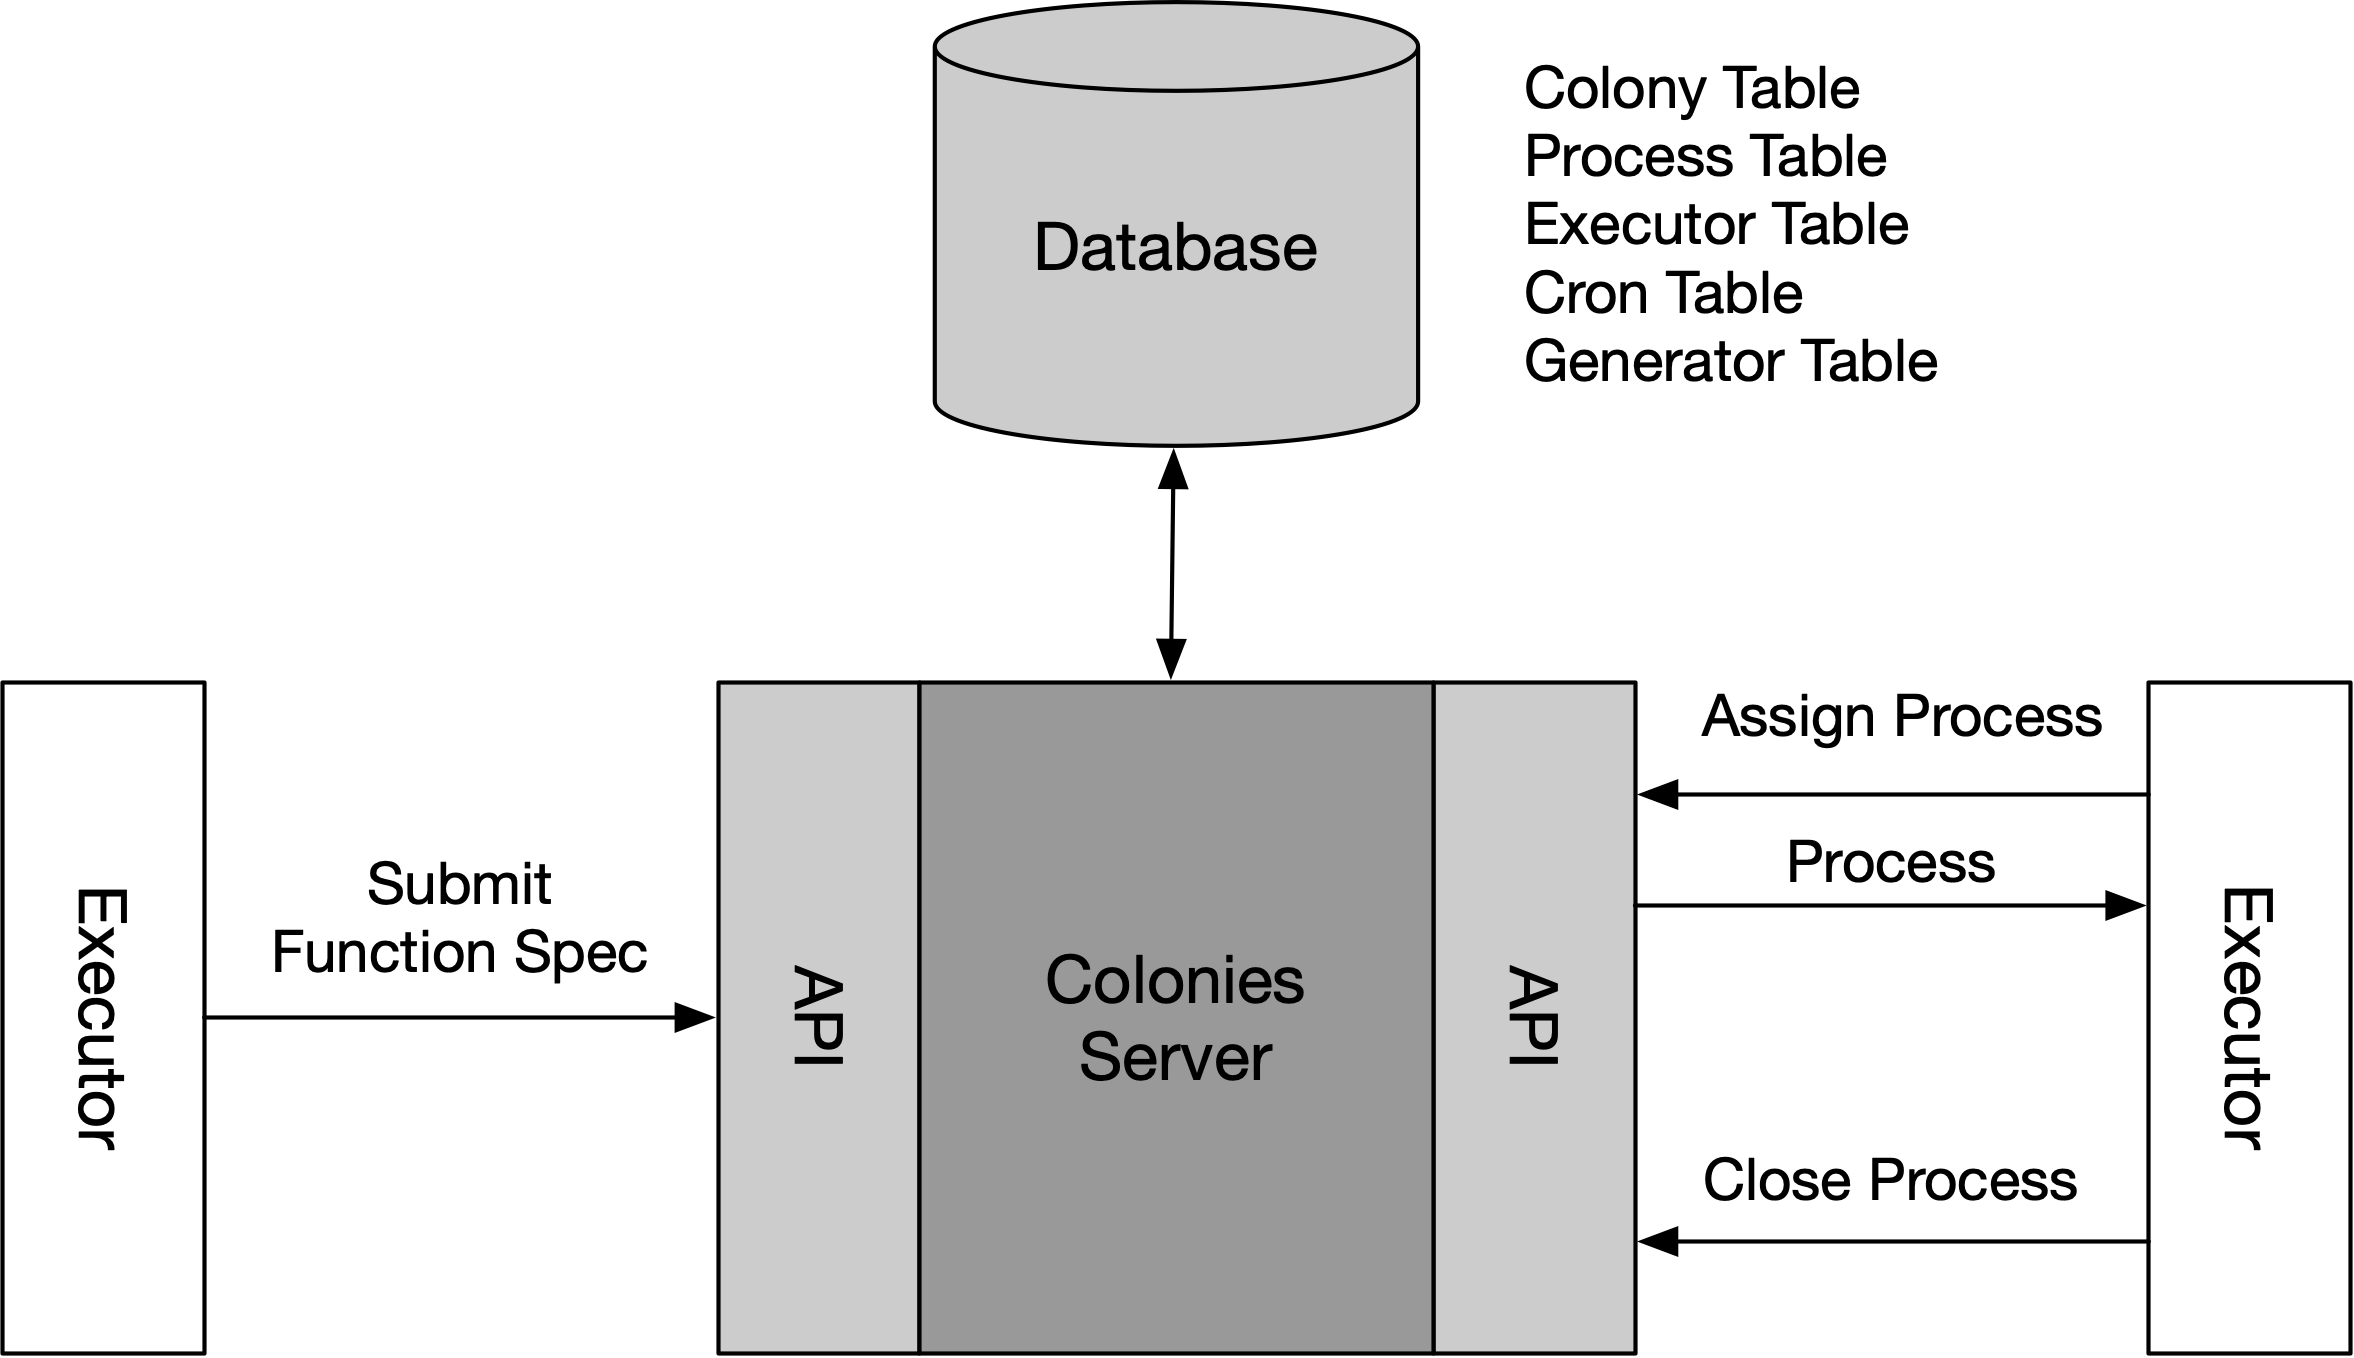
\includegraphics[scale=0.39]{arch.png}
         \caption{Process assignment steps.}
         \label{fig:y equals x}
     \end{subfigure}
     \hfill
     \begin{subfigure}[b]{0.3\textwidth}
         \centering
         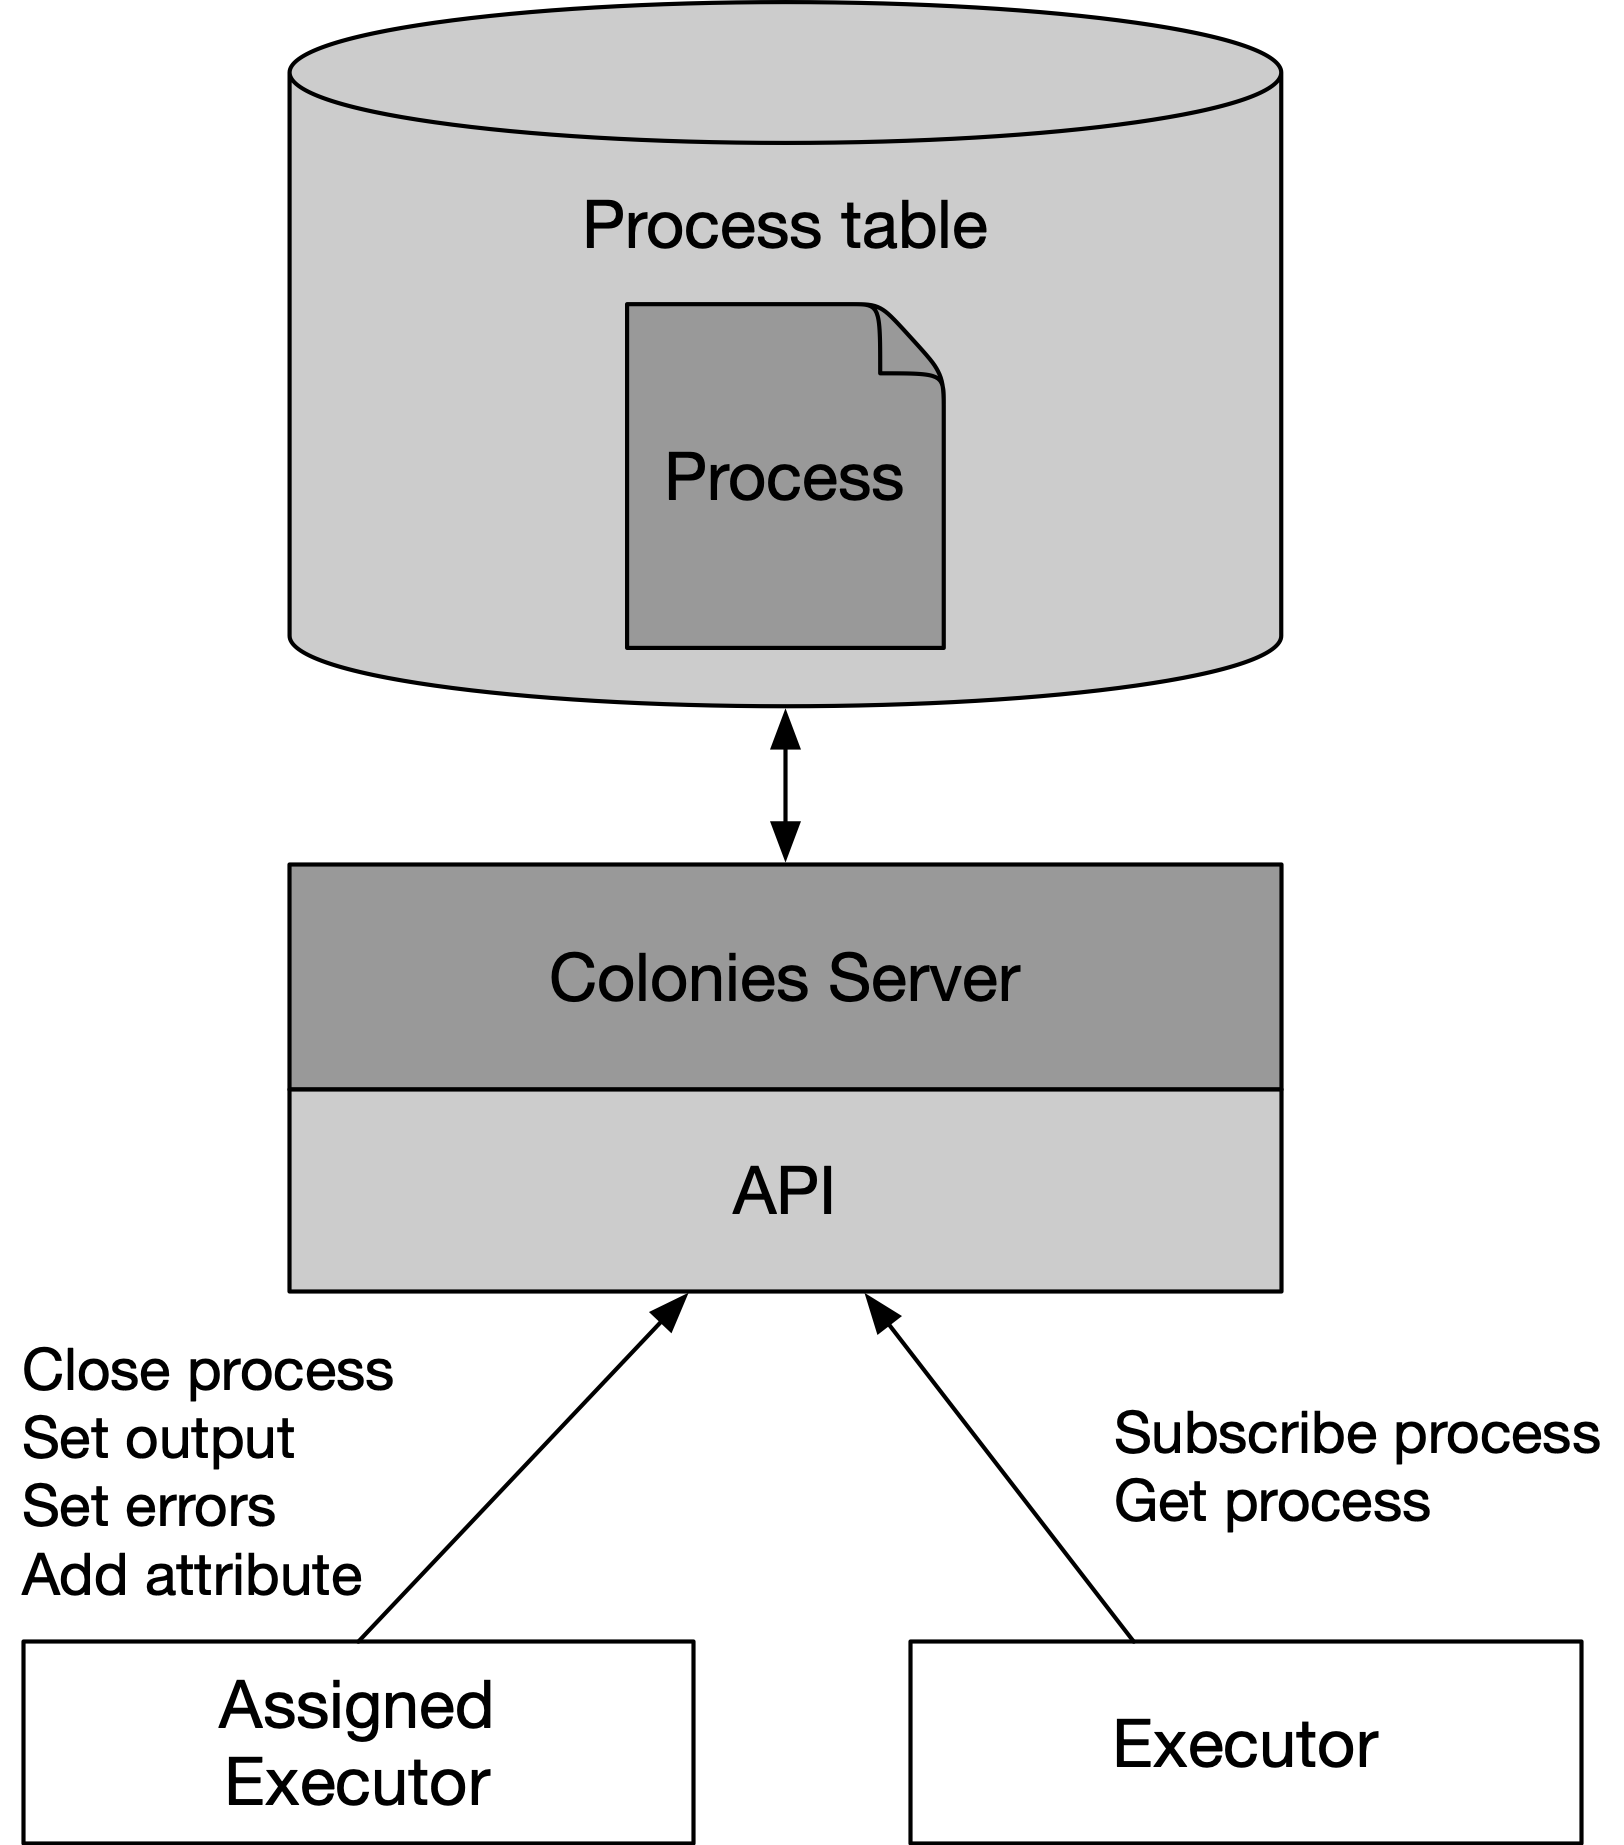
\includegraphics[scale=0.39]{process.png}
         \caption{Manipulation of a process.}
         \label{fig:three sin x}
     \end{subfigure}
     \caption{Process management via Colonies HTTP API. Note that only the assigned executor has write access to the process database entry.}
     \label{fig:three graphs}
\end{figure}

\subsection{Process tables}
Colonies provides a platform for executors to interact with each other by enabling them to submit function specifications to a Colonies server. Once submitted, other executors can connect to the server to receive execution assignments. When a function specification is submitted to the Colonies server, it is store as a process entry in a dedicated process table database. In this case, a process is analogous to a task, but contains additional contextual information about the execution, for example, execution status (waiting, running, successful, failed), assigned executor Id, submission time, execution time, deadlines, priority etc. It also contains input and argument values as well as return values from the function innovation.

The Colonies server acts as a job broker for executors, almost like an employment agency. When an executor connects to the Colonies server, the server hang the incomming HTTP connection\footnote{An alternative protocol is to use WebSockets or gPRC to communicate with the Colonies server.} until the executor is assigned a process, or until a connection timer expires. Note that the Colonies server does not connect to any executor. Rather, it is the responsibility of the executors to connect to the Colonies server, enabling them to be deployed anywhere on the Internet, even behind firewalls or commercial telco networks.

Figure \ref{fig:fig1} illustrates an executor submitting a function specification that is later assigned to another executor. Executors have to specify to the Colonies server which functions they are capable of executing. The Colonies server makes sure that the conditions (or requirmenets) of a function specification matches the capability of the executors. 

\begin{figure}[h]
	\centering
    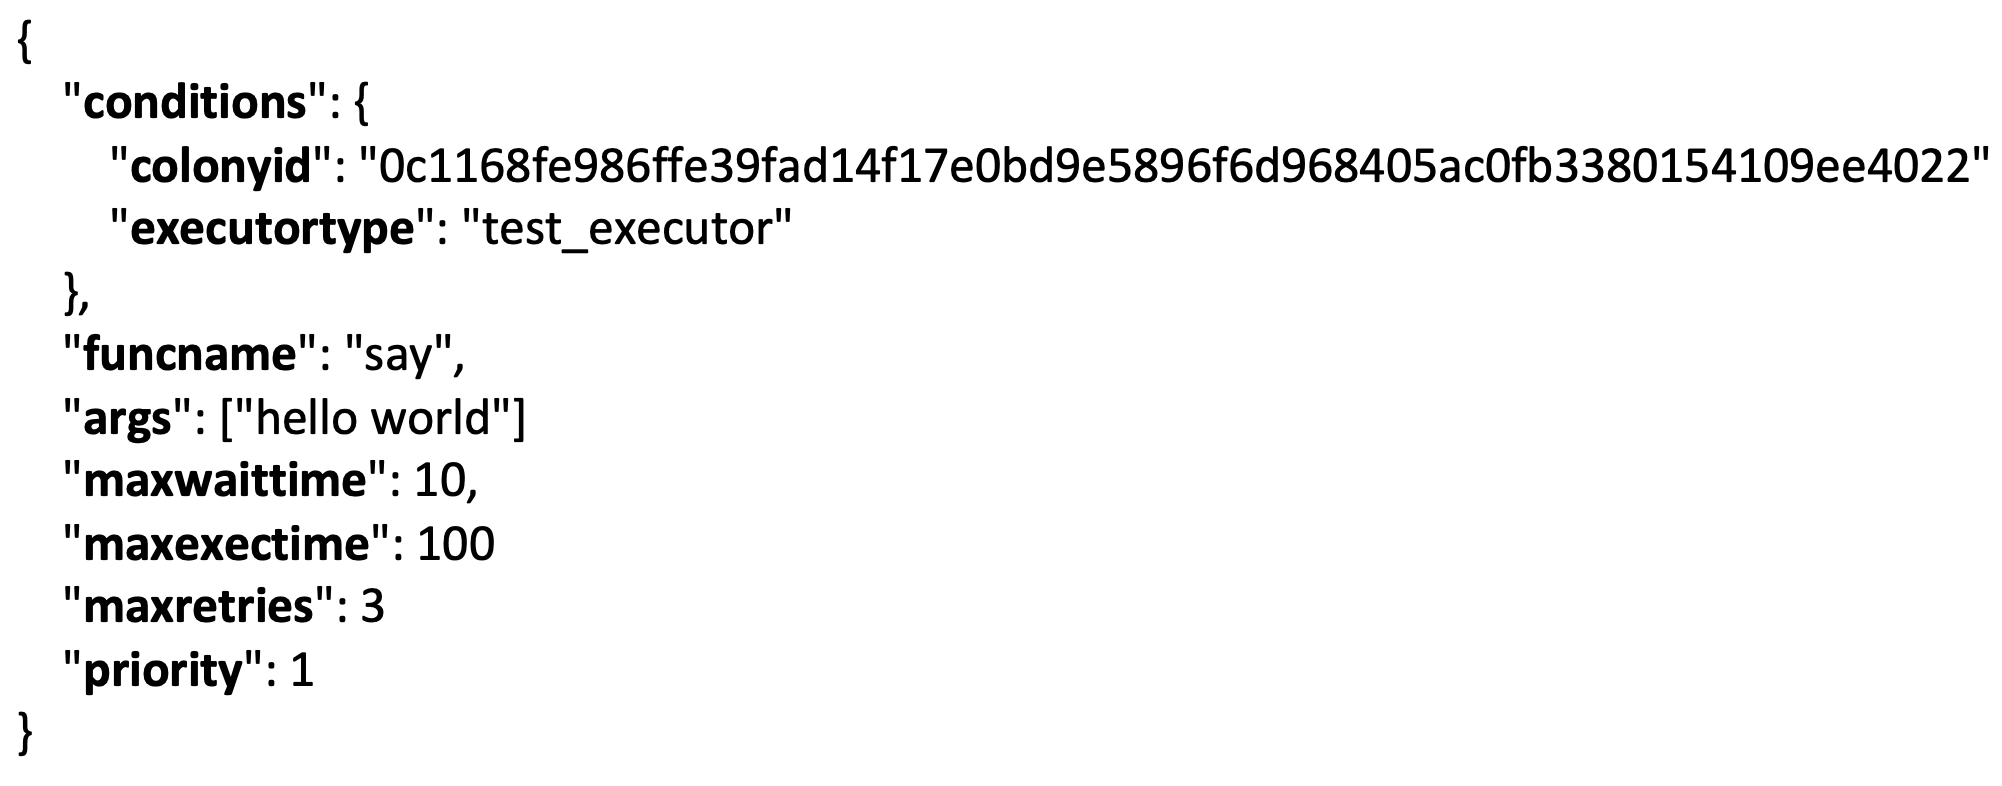
\includegraphics[scale=0.35]{function_spec.png}
	\caption{Example of a function spec.}
	\label{fig:fig2}
\end{figure}

Figure \ref{fig:fig2} shows an example of a function specification. The \emph{maxexectime} attribute specifies the maximum time an executor may run a process (in this case, 100 seconds). Before a process is assigned to an executor, the Colonies server updates the process entry in the process table database and calculates a deadline for when the process must be finished. The server then regularly checks for any running processes that have exceeded their deadlines. If such process is detected, it is reset, allowing it to be re-assigned to other executors. This scheme is completely stateless, so if the Colonies server crashes, another Colonies server can take over and look for processes that have exceeded their deadline. Moreover, if an executor assigned to a process crashes, the process is simply re-executed by another executor.

To scale up a system, more executors can be deployed. Scaling down, however, can be more challenging. One solution is to select a set of executors to be removed and then starv them out by denying them new process assignments. Another, simpler solution, is to immediately destroy the executors, or if possible notify them in advance so that they can gracefully unregister. 

The \emph{maxexectime} failsafe mechanism ensures that processes will eventually be executed even in the case of failures. This mechanism also relieves the burden of user to check if a process has been executed or not, as they can simply look up the process in the database to get its current status. It is also possible to subscribe on process changhes using an event-driven protocol, but this may be impractical if a process runs for a very long time (e.g. days or weeks).

\begin{figure}[h]
	\centering
    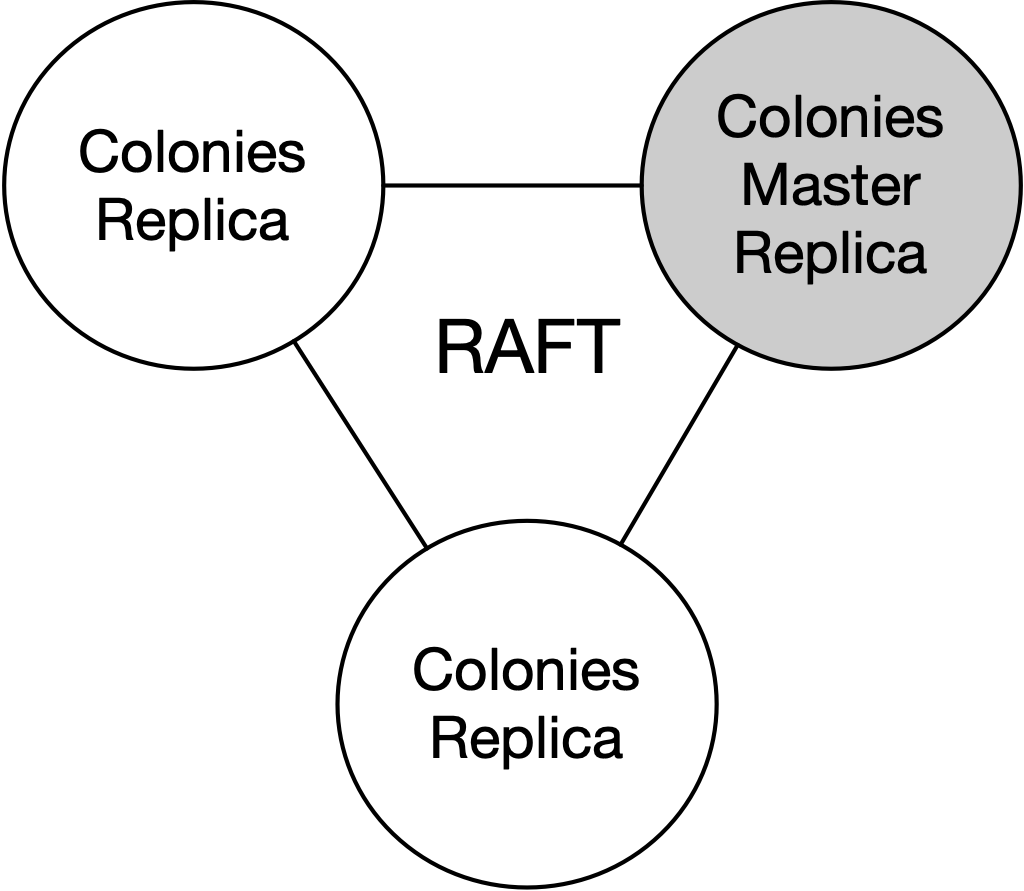
\includegraphics[scale=0.4]{raft.png}
	\caption{cron management}
	\label{fig:fig2}
\end{figure}

\subsubsection{Concurreny and synchronization}
Synchronization is esstential to prevent data inconsistency and race conditions when accessing shared resources concurrently with multiple threads. However, synchronization also slows down execution as only one thread can access critical sections at a time. By carefully designing multithreaded applications and employing the right synchronization techniques, it possible to minimize the performance impact while still ensuring data consistency and correctness.  

The purpose of all Colonies APIs is to either modify the database or read information from the database. A request 

Colonies is designed to be stateless, meaning that the Colonies server does not keep any information about between API requests. In other words, each request is handled independently, without relying on any information from previous requests. Once the database has been updated,

if an instance fails or becomes unavailable, subsequent requests can be easily redirected to another

. After a The Colonies server ensure that only the assigned executor has write access to the process entry in the database. 

Colonies ensures that exactly one executor is assigned to a specific process, so only the assigned executor has permission to set output values and close the process as successful. However, there is a window of time during which an executor may execute a process.

\subsubsection{Workflows}
TODO
\begin{figure}[h]
	\centering
    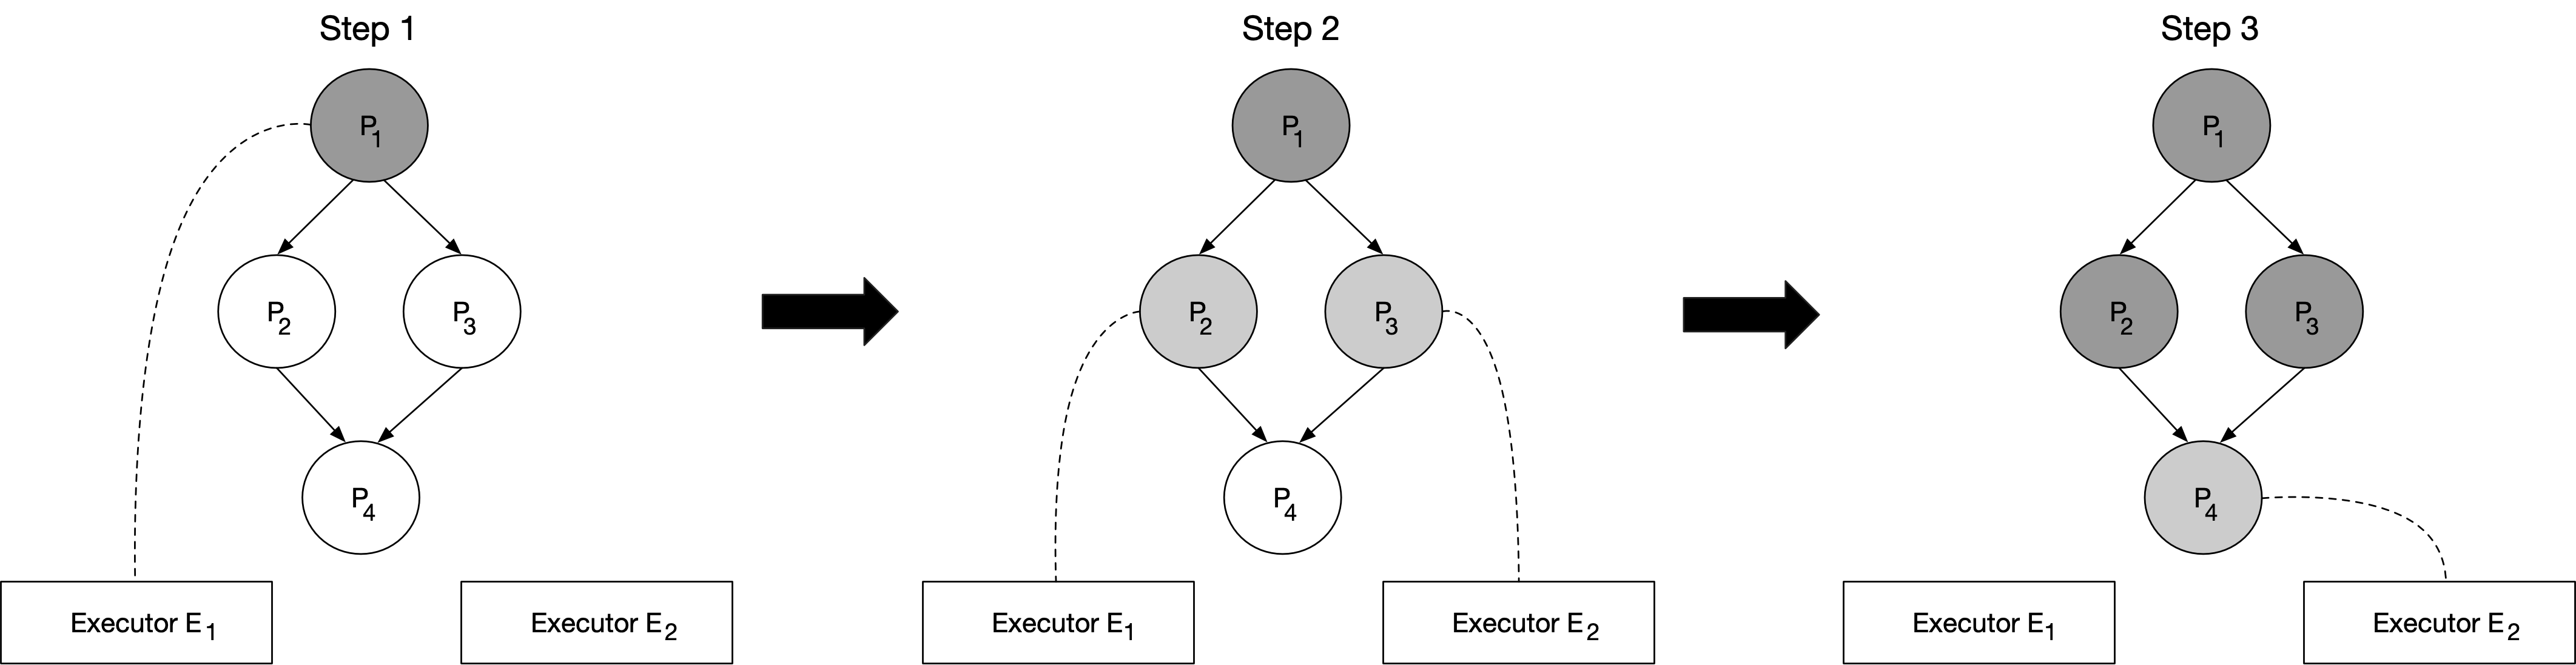
\includegraphics[scale=0.32]{workflow.png}
	\caption{cron management}
	\label{fig:fig3}
\end{figure}

\begin{table}[h]
	\caption{Function Specifications}
	\centering
	\begin{tabular}{llllll}
		\toprule
		\cmidrule(r){1-2}
        Function Spec & Function        & Executor Type & Priority & Max Exec Time & Max Retries \\
		\midrule
        $F_{1}$       & gen\_nums()     & Edge          & 1        & 200 s         & 5 \\
        $F_{2}$       & square()        & Cloud         & 1        & 200 s         & 5 \\
        $F_{3}$       & square()        & Cloud         & 1        & 200 s         & 5 \\
        $F_{4}$       & sum()           & Browser       & 1        & 200 s         & 5 \\
		\bottomrule
	\end{tabular}
	\label{tab:table}
\end{table}

\begin{table}[h]
	\caption{Snapshot of Process Table as in Step 2}
	\centering
	\begin{tabular}{llllll}
		\toprule
		\cmidrule(r){1-2}
        Process Id & Function Spec & Wait for Parents & Assigned Executor Id & State      & Priority Time \\
		\midrule
        $P_{1}$    & $F_{1}$       & $False$          & $E_{1}$              & Successful & 1679906715352024000 \\
        $P_{2}$    & $F_{2}$       & $False$          & $E_{1}$              & Running    & 1679906715353453000 \\
        $P_{3}$    & $F_{3}$       & $False$          & $E_{2}$              & Running    & 1679906715354286000 \\
        $P_{4}$    & $F_{4}$       & $True$           & -                    & Waiting    & 1679906715355188000 \\
		\bottomrule
	\end{tabular}
	\label{tab:table}
\end{table}

dt = -1000000000 * 60 * 60 * 24
process.PriorityTime = int64(process.FunctionSpec.Priority)*dt + submissionTime.UnixNano()


\begin{table}[h]
	\caption{Dependency Table}
	\centering
	\begin{tabular}{lll}
		\toprule
		\cmidrule(r){1-2}
        Process Id & Name       & Dependencies           \\
		\midrule
        $P_{1}$    & $Task_{1}$ & -                      \\
        $P_{2}$    & $Task_{2}$ & $Task_{1}$             \\
        $P_{3}$    & $Task_{3}$ & $Task_{1}$             \\
        $P_{4}$    & $Task_{4}$ & $Task_{2}$, $Task_{3}$ \\
		\bottomrule
	\end{tabular}
	\label{tab:table}
\end{table}
	
\begin{table}[h]
	\caption{Input/Output Table}
	\centering
	\begin{tabular}{lll}
		\toprule
		\cmidrule(r){1-2}
        Process Id & Input & Output \\
		\midrule
        $P_{1}$    & & [2,3] \\
        $P_{2}$    & 2 & 4 \\
        $P_{3}$    & 3 & 9 \\
        $P_{4}$    & [4,9] & 13 \\
		\bottomrule
	\end{tabular}
	\label{tab:table}
\end{table}

\subsubsection{Cron}
TODO
\begin{figure}[h]
	\centering
    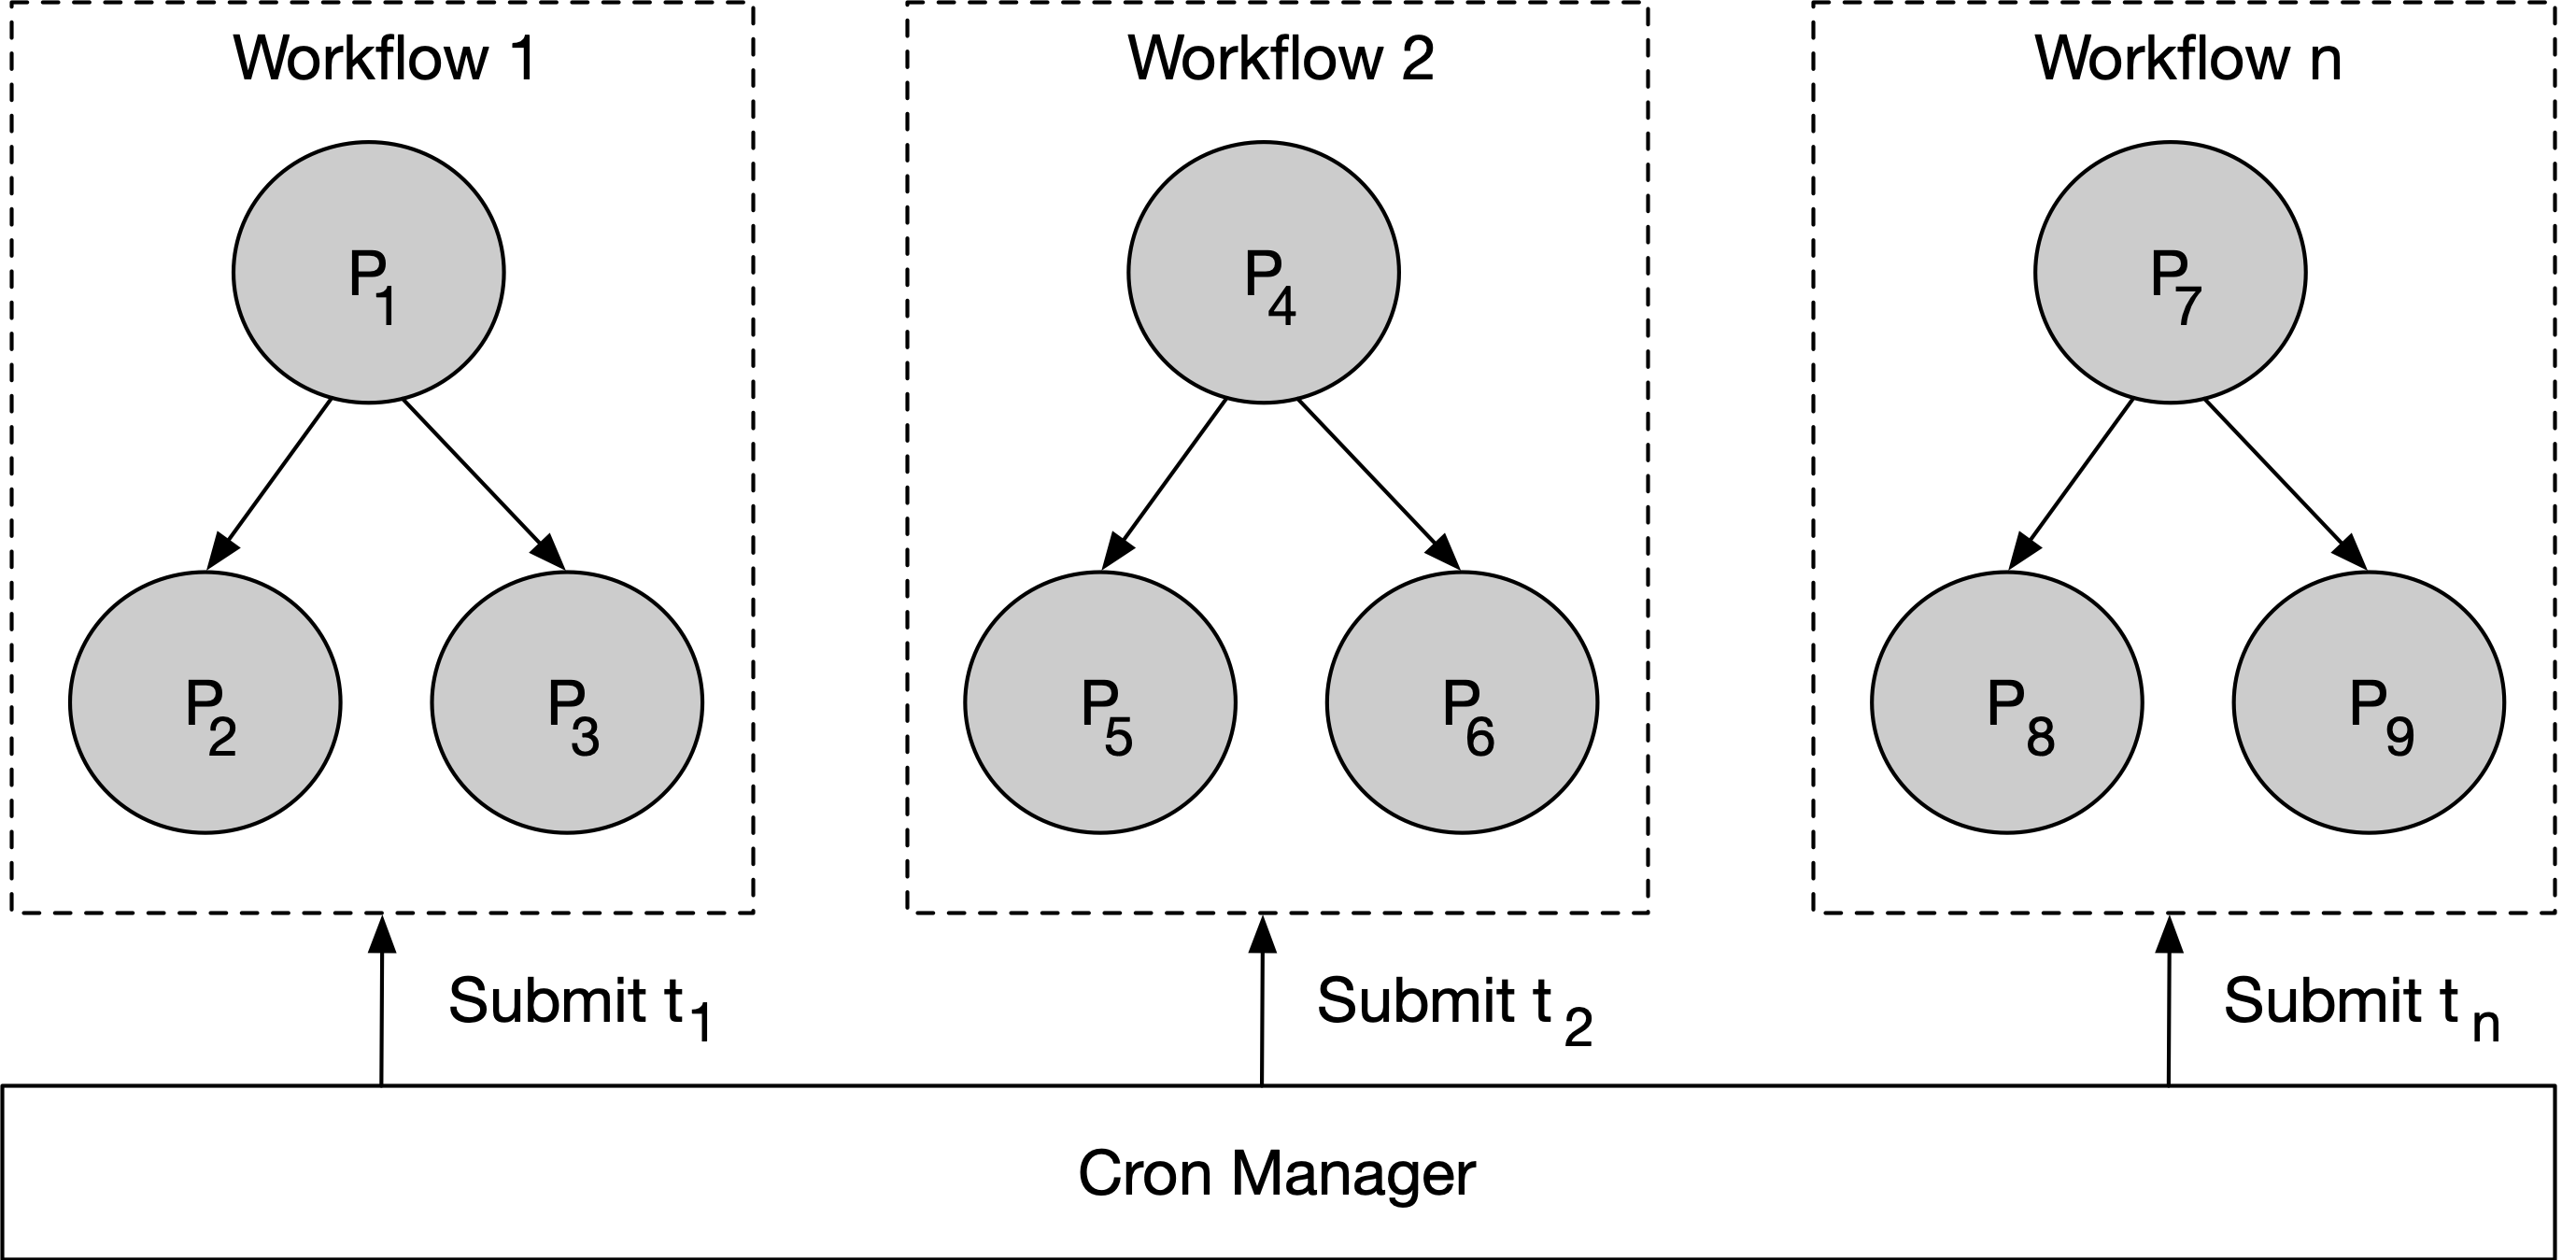
\includegraphics[scale=0.4]{cron.png}
	\caption{Sample figure caption.}
	\label{fig:fig1}
\end{figure}

\subsubsection{Generators}
TODO

\subsubsection{Zero-trust security}
TODO

\section{Evaluation}
\subsection{Implementation}
\begin{lstlisting}[language=c]
gen_nums = Function(gen_data, colonyid, executortype="edge")
square1 = Function(square, colonyid, executortype="cloud")
square2 = Function(square, colonyid, executortype="cloud")
sum = Function(square, colonyid, executortype="browser")

wf = ColoniesWorkflow("localhost", 50080, colonyid, executor_prvkey)
wf >> gennums
gennums >> square1
gennums >> square2
[square1, square2] >> sum
res = wf.execute()
\end{lstlisting}

\subsection{References}
TODO
\bibliographystyle{unsrtnat}
\bibliography{references}  %%% Uncomment this line and comment out the ``thebibliography'' section below to use the external .bib file (using bibtex) .


%%% Uncomment this section and comment out the \bibliography{references} line above to use inline references.
% \begin{thebibliography}{1}

% 	\bibitem{kour2014real}
% 	George Kour and Raid Saabne.
% 	\newblock Real-time segmentation of on-line handwritten arabic script.
% 	\newblock In {\em Frontiers in Handwriting Recognition (ICFHR), 2014 14th
% 			International Conference on}, pages 417--422. IEEE, 2014.

% 	\bibitem{kour2014fast}
% 	George Kour and Raid Saabne.
% 	\newblock Fast classification of handwritten on-line arabic characters.
% 	\newblock In {\em Soft Computing and Pattern Recognition (SoCPaR), 2014 6th
% 			International Conference of}, pages 312--318. IEEE, 2014.

% 	\bibitem{hadash2018estimate}
% 	Guy Hadash, Einat Kermany, Boaz Carmeli, Ofer Lavi, George Kour, and Alon
% 	Jacovi.
% 	\newblock Estimate and replace: A novel approach to integrating deep neural
% 	networks with existing applications.
% 	\newblock {\em arXiv preprint arXiv:1804.09028}, 2018.

% \end{thebibliography}

\end{document}
